\subsubsection{UC3 - Amministrazione di sistema}
	\begin{center}
		\begin{figure}[h!]
			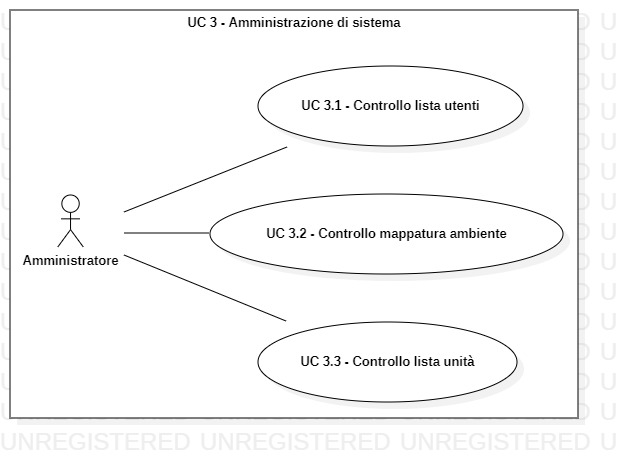
\includegraphics[width=5cm]{res/img/firme/uc3.jpg}
			\caption{Diagramma UC3}
		\end{figure}
	\end{center}
	\begin{itemize}
		\item \textbf{Attori primari:} utente amministratore;
		\item \textbf{Descrizione:} l'amministratore intende visualizzare le componenti del sistema, ed apportare le modifiche volute;
		\item \textbf{Scenario principale:} 
			\begin{itemize}
				\item l'amministratore gestisce la lista utenti (UC3.1);
				\item l'amministratore gestisce la mappatura dell'ambiente (UC3.2);
				\item l'amministratore gestisce la lista unità (UC3.3).
			\end{itemize}
		\item \textbf{Precondizione:} l'amministratore ha accesso alle componenti del sistema;
		\item \textbf{Postcondizione:} le componenti del sistema, rispetto al loro stato iniziale, risultano modificate come voluto.
	\end{itemize}
	
\subsubsection{UC3.1 - Gestione lista utenti}
	\begin{center}
		\begin{figure}[h!]
			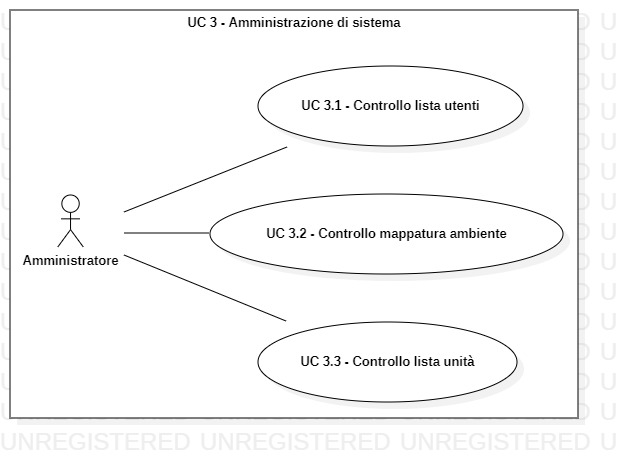
\includegraphics[width=5cm]{res/img/firme/uc3.jpg}
			\caption{Diagramma UC3.1}
		\end{figure}
	\end{center}
	\begin{itemize}
		\item \textbf{Attori primari:} utente amministratore;
		\item \textbf{Descrizione:} l'amministratore visiona la lista degli utenti che hanno accesso al sistema, ed applica le modifiche volute;
		\item \textbf{Scenario principale:} 
			\begin{itemize}
				\item l'amministratore inserisce un utente (UC3.1.1);
				\item l'amministratore modifica un utente (UC3.1.2);
				\item l'amministratore elimina un utente (UC3.1.3).
			\end{itemize}
		\item \textbf{Precondizione:} l'amministratore visualizza l'elenco degli utenti esistenti;
		\item \textbf{Postcondizione:} la lista degli utenti, rispetto allo stato iniziale, risulta modificata come voluto.
	\end{itemize}

\subsubsection{UC3.1.1 - Inserimento utente}
\begin{itemize}
	\item \textbf{Attori primari:} utente amministratore;
	\item \textbf{Descrizione:} l'amministratore intende aggiungere un nuovo utente, alla lista degli utenti che hanno accesso al sistema;
	\item \textbf{Scenario principale:} l'amministratore inserisce le credenziali dell'utente interessato alla lista di quelli già esistenti;
	\item \textbf{Precondizione:} l'amministratore visualizza l'elenco degli utenti esistenti;
	\item \textbf{Postcondizione:} la lista degli utenti risulta aggiornata con l'aggiunta dell'utente interessato.
\end{itemize}

\subsubsection{UC3.1.2 - Modifica utente}
\begin{itemize}
	\item \textbf{Attori primari:} utente amministratore;
	\item \textbf{Descrizione:} l'amministratore intende modificare le credenziali di un utente già esistente;
	\item \textbf{Scenario principale:} l'amministratore modifica le credenziali dell'utente interessato, presente nella lista degli utenti;
	\item \textbf{Precondizione:} l'amministratore visualizza l'elenco degli utenti esistenti;
	\item \textbf{Postcondizione:} le credenziali dell'utente interessato risultano aggiornate come voluto.
\end{itemize}

\subsubsection{UC3.1.3 - Rimozione utente}
\begin{itemize}
	\item \textbf{Attori primari:} utente amministratore;
	\item \textbf{Descrizione:} l'amministratore intende eliminare utente dalla lista degli utenti che hanno accesso al sistema;
	\item \textbf{Scenario principale:} l'amministratore cancella l'utente interessato dalla lista degli utenti;
	\item \textbf{Precondizione:} l'amministratore visualizza l'elenco degli utenti esistenti;
	\item \textbf{Postcondizione:} la lista degli utenti risulta aggiornata con la rimozione dell'utente interessato.
\end{itemize}

\subsubsection{UC3.2 - Gestione mappatura ambiente}
	\begin{center}
		\begin{figure}[h!]
			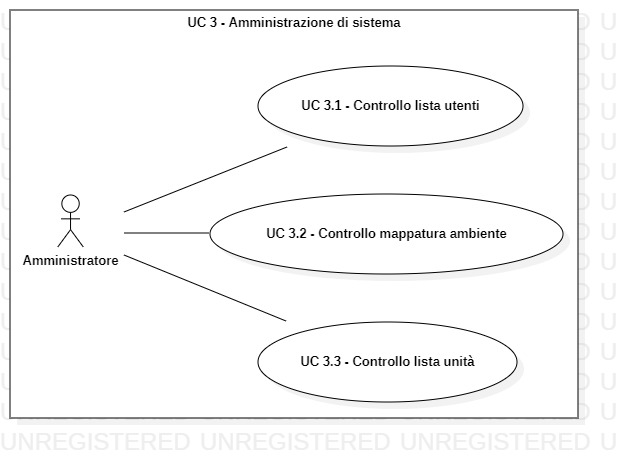
\includegraphics[width=5cm]{res/img/firme/uc3.jpg}
			\caption{Diagramma UC3.2}
		\end{figure}
	\end{center}
	\begin{itemize}
		\item \textbf{Attori primari:} utente amministratore;
		\item \textbf{Descrizione:} l'amministratore visiona la mappatura dell'ambiente, ed applica le modifiche volute;
		\item \textbf{Scenario principale:} l'amministratore modifica la mappatura dell'ambiente gestito dal sistema;
		\item \textbf{Precondizione:} l'amministratore visualizza lo stato attuale della mappa;
		\item \textbf{Postcondizione:} la mappa, rispetto allo stato iniziale, risulta modificata come voluto.
	\end{itemize}

\subsubsection{UC 3.2.1 - !!!!!!!!!!!!!!!!!!!!!!!!!!}
\begin{itemize}
	\item \textbf{Attori primari:} utente amministratore;
	\item \textbf{Descrizione:} ;
	\item \textbf{Scenario principale:} 
	\item \textbf{Precondizione:} ;
	\item \textbf{Postcondizione:} .
\end{itemize}

\subsubsection{UC3.3 - Gestione lista unità}
	\begin{center}
		\begin{figure}[h!]
			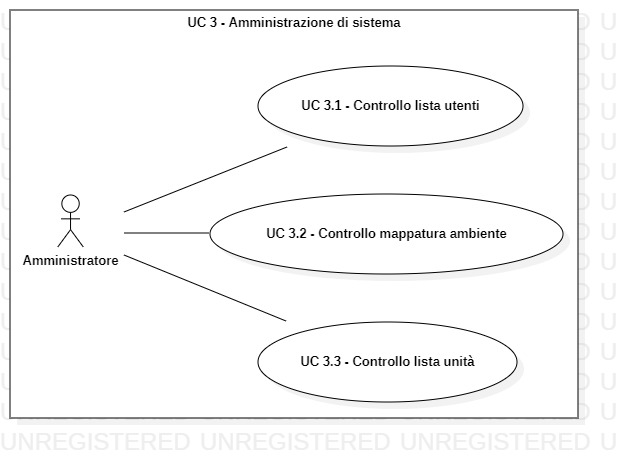
\includegraphics[width=5cm]{res/img/firme/uc3.jpg}
			\caption{Diagramma UC3.3}
		\end{figure}
	\end{center}
	\begin{itemize}
		\item \textbf{Attori primari:} utente amministratore;
		\item \textbf{Descrizione:} l'amministratore visiona la lista delle unità presenti nel sistema, ed applica le modifiche volute;
		\item \textbf{Scenario principale:} 
			\begin{itemize}
				\item l'amministratore inserisce un'unità (UC3.3.1);
				\item l'amministratore modifica un'unità (UC3.3.2);
				\item l'amministratore elimina un'unità (UC3.3.3).
			\end{itemize}
		\item \textbf{Precondizione:} l'amministratore visualizza l'elenco delle unità esistenti;
		\item \textbf{Postcondizione:} la lista delle unità risulta modificata come voluto rispetto allo stato iniziale.
	\end{itemize}

\subsubsection{UC3.3.1 - Inserimento unità}
\begin{itemize}
	\item \textbf{Attori primari:} utente amministratore;
	\item \textbf{Descrizione:} l'amministratore intende aggiungere una nuova unità, alla lista di quelle gestite dal sistema;
	\item \textbf{Scenario principale:} l'amministratore aggiunge l'unità interessata alla lista di quelle già esistenti;
	\item \textbf{Precondizione:} l'amministratore visualizza l'elenco delle unità esistenti;
	\item \textbf{Postcondizione:} la lista delle unità risultà aggiornata con l'aggiunta dell'unità interessata.
\end{itemize}

\subsubsection{UC3.3.2 - Modifica unità}
\begin{itemize}
	\item \textbf{Attori primari:} utente amministratore;
	\item \textbf{Descrizione:} l'amministratore intende modificare le proprietà di un'unità già esistente;
	\item \textbf{Scenario principale:} l'amministratore modifica le proprietà dell'unità interessata;
	\item \textbf{Precondizione:} l'amministratore visualizza l'elenco delle unità esistenti;
	\item \textbf{Postcondizione:} le proprietà dell'unità interessata risultano aggiornate come voluto.
\end{itemize}

\subsubsection{UC3.3.3 - Rimozione unità}
\begin{itemize}
	\item \textbf{Attori primari:} utente amministratore;
	\item \textbf{Descrizione:} l'amministratore intende eliminare un'unità, dalla lista di quelle gestite dal sistema;
	\item \textbf{Scenario principale:} l'amministratore cancella l'unità interessata dalla lista di quelle esistenti;
	\item \textbf{Precondizione:} l'amministratore visualizza l'elenco delle unità esistenti;
	\item \textbf{Postcondizione:} la lista delle unità risultà aggiornata con la rimozione dell'unità interessata.
\end{itemize}